\documentclass{article}
% Change "article" to "report" to get rid of page number on title page
\usepackage{amsmath,amsfonts,amsthm,amssymb}
\usepackage{setspace}
\usepackage{Tabbing}
\usepackage{fancyhdr}
\usepackage{lastpage}
\usepackage{extramarks}
\usepackage{chngpage}
\usepackage{soul,color}
\usepackage{graphicx,float,wrapfig}
\usepackage{multirow}
\usepackage{enumerate}
% In case you need to adjust margins:
\topmargin=-0.45in      %
\evensidemargin=0in     %
\oddsidemargin=0in      %
\textwidth=6.5in        %
\textheight=9.0in       %
\headsep=0.25in         %

% Homework Specific Information
\newcommand{\hmwkTitle}{Finaally...Let there be bars!!!}
\newcommand{\hmwkClass}{}
\newcommand{\hmwkAuthorName}{Donglai\ Wei}


% Setup the header and footer
\pagestyle{fancy}                                                       %
\lhead{\hmwkAuthorName}                                                 %
\rhead{\firstxmark}                                                     %
\lfoot{\lastxmark}                                                      %
\cfoot{}                                                                %
\rfoot{Page\ \thepage\ of\ \pageref{LastPage}}                          %
\renewcommand\headrulewidth{0.4pt}                                      %
\renewcommand\footrulewidth{0.4pt}                                      %

% This is used to trace down (pin point) problems
% in latexing a document:
%\tracingall

%%%%%%%%%%%%%%%%%%%%%%%%%%%%%%%%%%%%%%%%%%%%%%%%%%%%%%%%\begin{enumerate}

% Some tools
\newcommand{\enterProblemHeader}[1]{\nobreak\extramarks{#1}{#1 continued on next page\ldots}\nobreak%
                                    \nobreak\extramarks{#1 (continued)}{#1 continued on next page\ldots}\nobreak}%
\newcommand{\exitProblemHeader}[1]{\nobreak\extramarks{#1 (continued)}{#1 continued on next page\ldots}\nobreak%
                                   \nobreak\extramarks{#1}{}\nobreak}%

\newlength{\labelLength}
\newcommand{\labelAnswer}[2]
  {\settowidth{\labelLength}{#1}%
   \addtolength{\labelLength}{0.25in}%
   \changetext{}{-\labelLength}{}{}{}%
   \noindent\fbox{\begin{minipage}[c]{\columnwidth}#2\end{minipage}}%
   \marginpar{\fbox{#1}}%

   % We put the blank space above in order to make sure this
   % \marginpar gets correctly placed.
   \changetext{}{+\labelLength}{}{}{}}%

\setcounter{secnumdepth}{0}
\newcommand{\homeworkProblemName}{}%
\newcounter{homeworkProblemCounter}%
\newenvironment{homeworkProblem}[1][Problem \arabic{homeworkProblemCounter}]%
  {\stepcounter{homeworkProblemCounter}%
   \renewcommand{\homeworkProblemName}{#1}%
   \section{\homeworkProblemName}%
   \enterProblemHeader{\homeworkProblemName}}%
  {\exitProblemHeader{\homeworkProblemName}}%

\newcommand{\problemAnswer}[1]
  {\noindent\fbox{\begin{minipage}[c]{\columnwidth}#1\end{minipage}}}%

\newcommand{\problemLAnswer}[1]
  {\labelAnswer{\homeworkProblemName}{#1}}

\newcommand{\homeworkSectionName}{}%
\newlength{\homeworkSectionLabelLength}{}%
\newenvironment{homeworkSection}[1]%
  {% We put this space here to make sure we're not connected to the above.
   % Otherwise the changetext can do funny things to the other margin

   \renewcommand{\homeworkSectionName}{#1}%
   \settowidth{\homeworkSectionLabelLength}{\homeworkSectionName}%
   \addtolength{\homeworkSectionLabelLength}{0.25in}%
   \changetext{}{-\homeworkSectionLabelLength}{}{}{}%
   \subsection{\homeworkSectionName}%
   \enterProblemHeader{\homeworkProblemName\ [\homeworkSectionName]}}%
  {\enterProblemHeader{\homeworkProblemName}%

   % We put the blank space above in order to make sure this margin
   % change doesn't happen too soon (otherwise \sectionAnswer's can
   % get ugly about their \marginpar placement.
   \changetext{}{+\homeworkSectionLabelLength}{}{}{}}%

\newcommand{\sectionAnswer}[1]
  {% We put this space here to make sure we're disconnected from the previous
   % passage

   \noindent\fbox{\begin{minipage}[c]{\columnwidth}#1\end{minipage}}%
   \enterProblemHeader{\homeworkProblemName}\exitProblemHeader{\homeworkProblemName}%
   \marginpar{\fbox{\homeworkSectionName}}%

   % We put the blank space above in order to make sure this
   % \marginpar gets correctly placed.
   }%

%%%%%%%%%%%%%%%%%%%%%%%%%%%%%%%%%%%%%%%%%%%%%%%%%%%%%%%%%%%%%



%%%%%%%%%%%%%%%%%%%%%%%%%%%%%%%%%%%%%%%%%%%%%%%%%%%%%%%%%%%%%
% Make title
\title{\vspace{0.3in}\textmd{\textbf{\hmwkTitle}}}
\date{2010.5.28}
\author{\textbf{\hmwkAuthorName}}
%%%%%%%%%%%%%%%%%%%%%%%%%%%%%%%%%%%%%%%%%%%%%%%%%%%%%%%%%%%%%

\begin{document}
\begin{spacing}{1.1}
\maketitle

\section{1) Key Ideas}

\begin{enumerate}
\item "Light-weighted" Grand-Split-Restaurant and Grand-Split-Dish with more runs 
\item modification f
\item 
\end{enumerate}



\begin{enumerate}[(I)]
 \item Initialization:\\
       \begin{enumerate}[(1)]
        \item Naive(bottom-up,top-down) 
        \item Auxilary Dishes
       \begin{enumerate}[(A)]
       \item Bottom-up:undesirable for large data setcounter
       \item {\bf Top-down:}
      \begin{enumerate}[(a)]
       \item split-table:Bad global maxima (Since auxilary dishes can be uninformative)
       \item approximation:{\bf greedy+drop t-term}
       \end{enumerate}
       \end{enumerate}
       \end{enumerate}

\item Search
   \begin{enumerate}[(1)]
     \item Stochastic search
     \item Big Moves
       \end{enumerate}

\end{enumerate}

\subsection{1.1) How does the restaurants look like}
\begin{figure}
    \centering 
    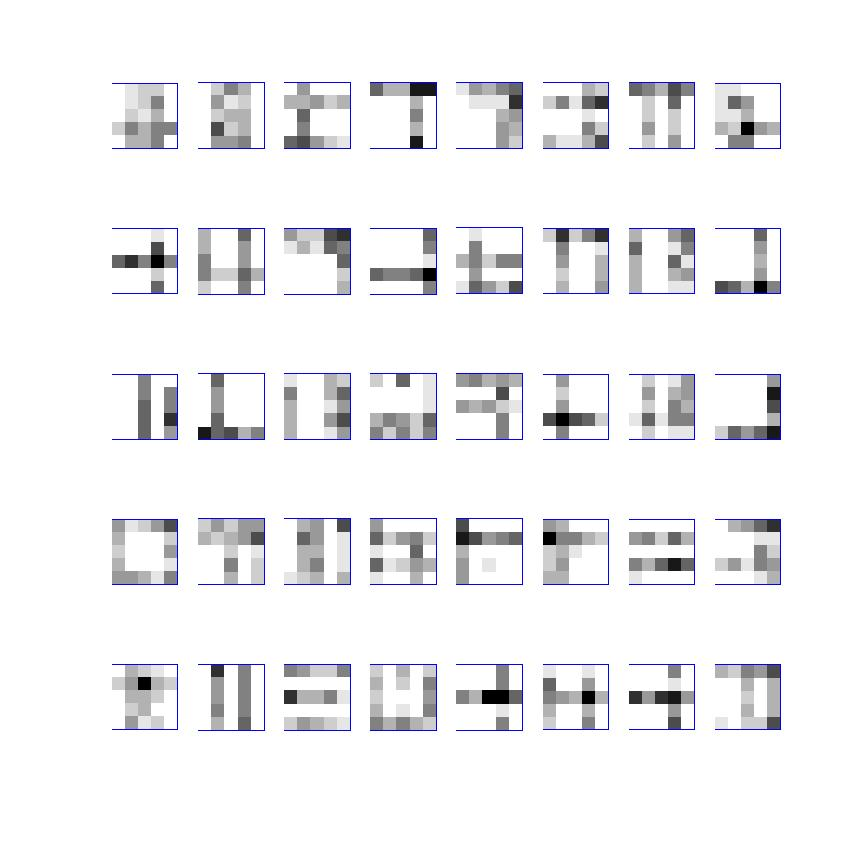
\includegraphics[width=7in,height=7in]{restau.jpg} 
    \caption{40 Restaurants}
\end{figure}

\section{2) Initialization}
\subsection{2.1) Split-table Can be BAD}
Below, I make 100 runs of split-table for the initialization(Auxilary Dishes) of Restaurant 1.\\ \\
Later, I checked that assign the whole restaurant to the second Auxilary Dish(Restaurant) is the global maxima.\\ \\
One rescue is to prune the Auxilary Dishes beforehand...But it can be tricky....\\ \\ \\ \\
\begin{figure}
    \centering 
    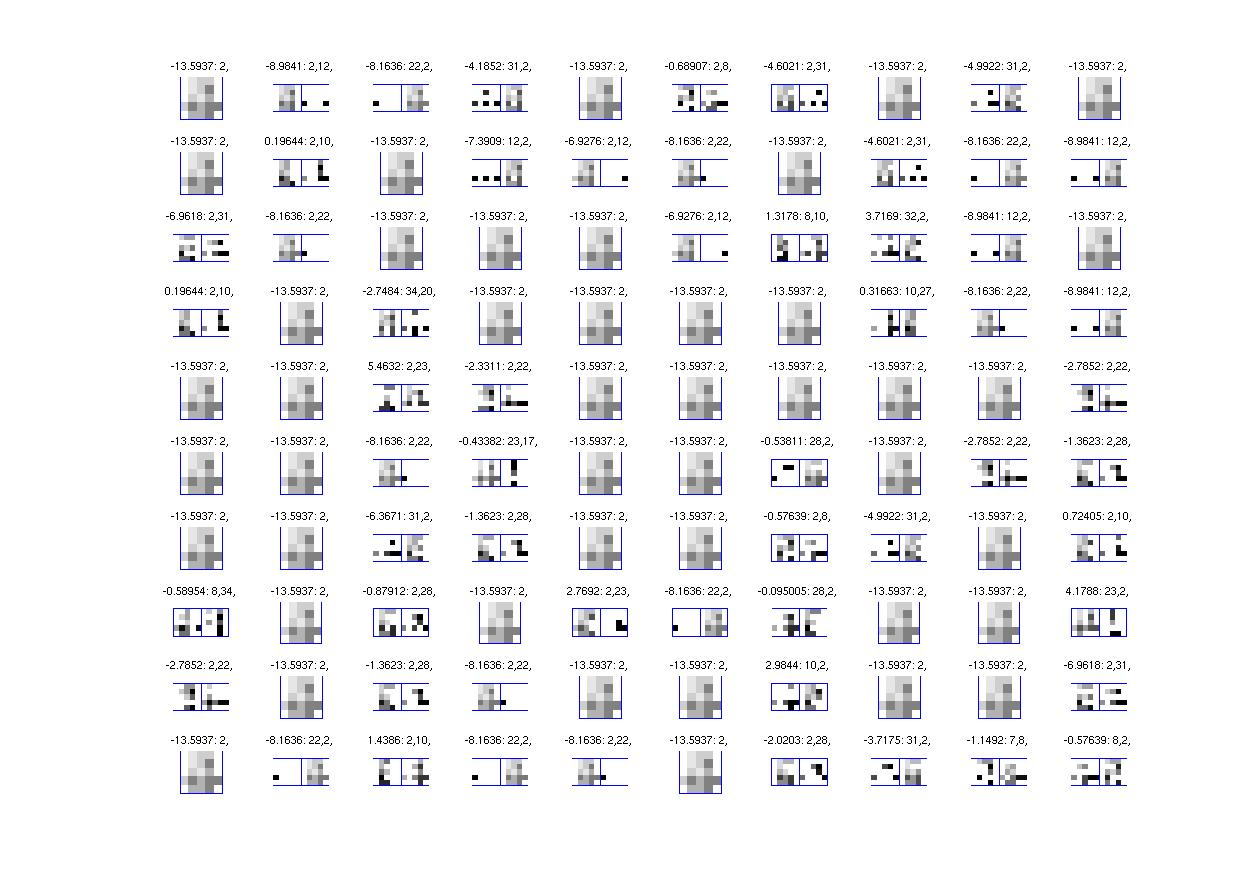
\includegraphics[width=7in,height=5in]{100_kmeans_2.jpg} 
    \caption{Initialization For the first Restaurant}
\end{figure}
\begin{figure}[h] 
  \begin{minipage}[b]{0.5\textwidth} 
    \centering 
    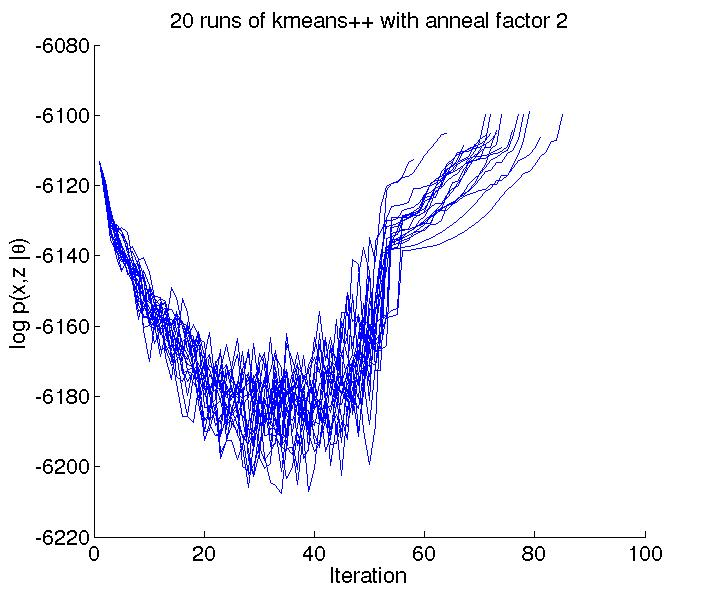
\includegraphics[width=3in,height=2in]{20_kmeans_2.jpg} 
    \caption{20 runs}
    \label{fig:by:table} 
  \end{minipage}% 
  \begin{minipage}[b]{0.5\textwidth} 
    \centering 
    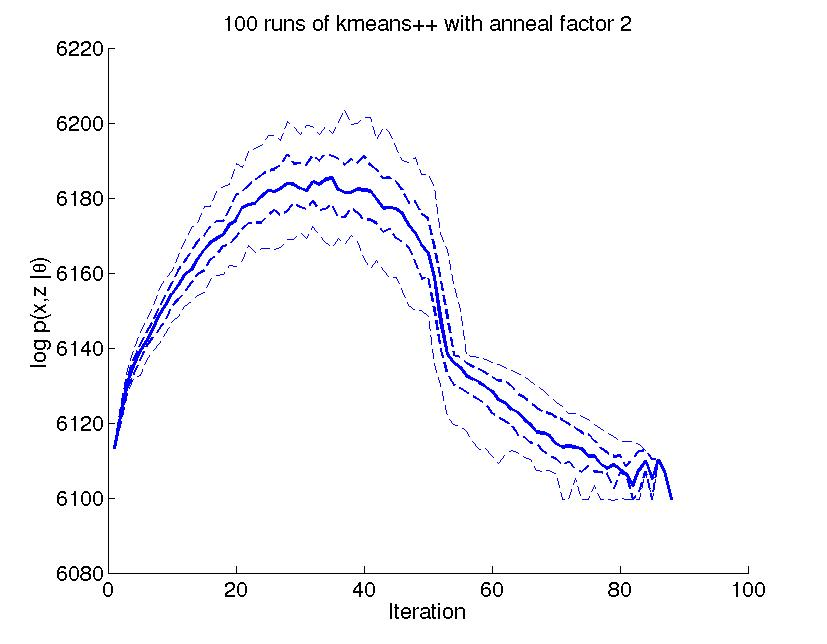
\includegraphics[width=3in,height=2in]{100_kmeans_2_q.jpg} 
    \caption{quantile for 100 runs}
    \label{fig:by:table}  
   \end{minipage}% 
\end{figure}
\begin{figure}
    \centering 
    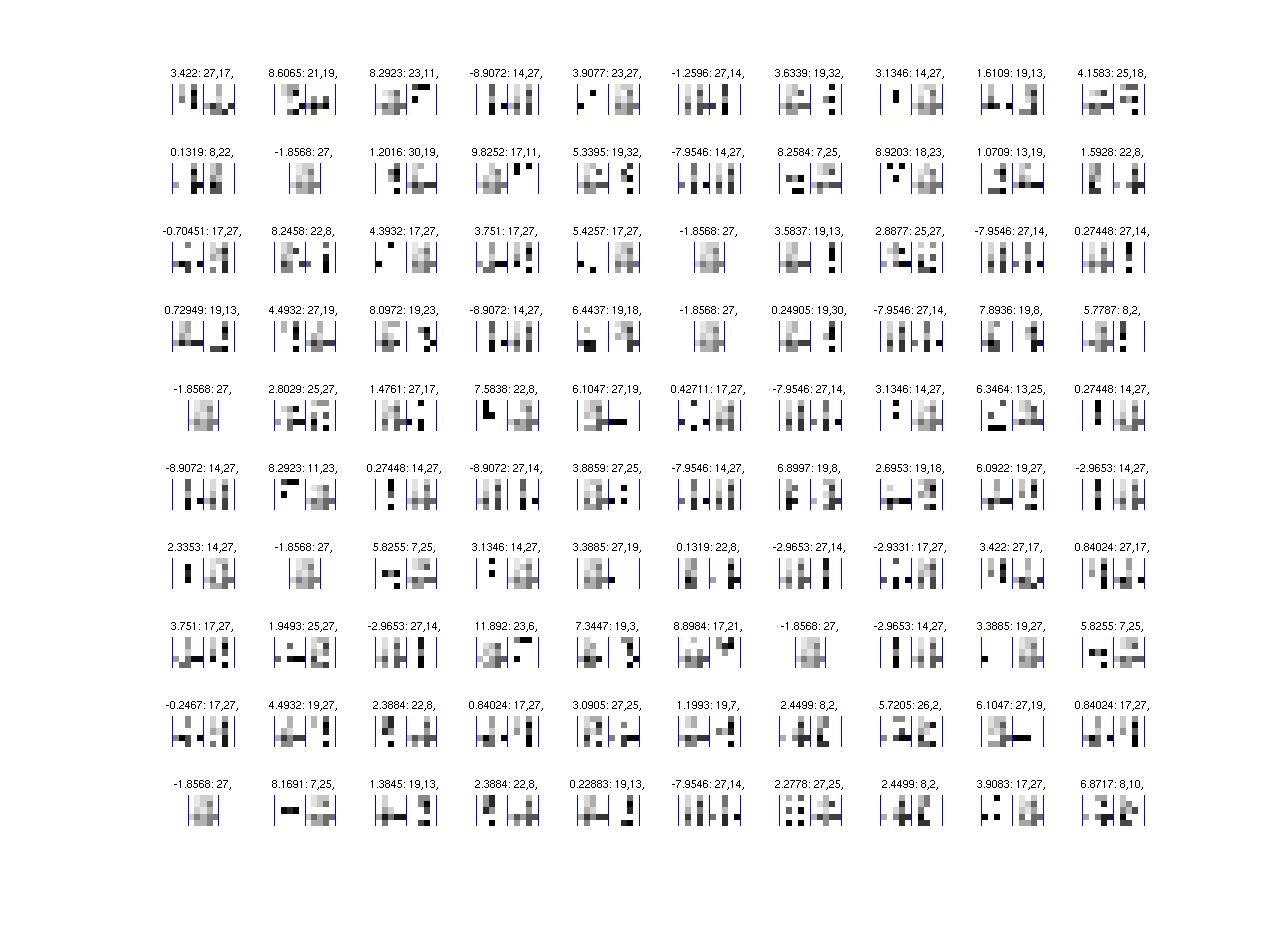
\includegraphics[width=7in,height=5in]{100_kmeans_prune.jpg} 
    \caption{Initialization after pruning}
\end{figure}

\subsection{2.2) Approximation}
For the initialization with Auxilary dishes, the {\bf Aim} is to find the table,dish configuration for the first Restaurant
to maximize the log likelihood:\\
$P=-log p(x,z|\lambda)$\\ =\\
(t-term)$ \underline{log \frac{\Gamma(m..+\gamma)}{\Gamma(\gamma)}+\sum_{j=1}^{J} \{log \frac{\Gamma(n_{j..}+\alpha)}{\Gamma(\alpha)}-\sum_{t=1}^{m_{j.}}[log(\Gamma(n_{jt.})+log \alpha
]\}}$\\ \\
+(k-term)$ \sum_{k=1}^{K} [log(\frac{\Gamma(n_{..k}+W\phi_{0})}{\Gamma(W\phi_{0})})+log(\Pi_{w=1}^{W}\frac{\Gamma(\phi_{0})}{\Gamma(\phi_{0}+n_{..k}^{w})})
-\underline{log(\Gamma(m_{.k})-log \gamma]}$\\ W:number of unique words\\ 
$n_{..k}^{w}$number of occurence of word w in dish k \\ \\ \\ 
Below are the sub-problems:\\
1)$m_{j}=1$:\\merge it to Restaurant q\\
$\delta P=log(\frac{\Gamma(n_{j..}+n_{q..}+W\phi_{0})}{\Gamma(n_{j..}+W\phi_{0})\Gamma(n_{q..}+W\phi_{0})})+log(\Pi_{w=1}^{W}\frac{\Gamma(\phi_{0}+n_{j..}^{w})\Gamma(\phi_{0}+n_{q..}^{w})}{\Gamma(\phi_{0}+n_{j..}^{w}+n_{q..}^{w})})$\\ \\
2)$m_{j}=2$:\\merge it to Restaurant p,q\\
$\delta P=\underline{log(m..+\gamma)+log(\frac{\Gamma(n_{j2.}+\alpha)}{\Gamma(n_{j1.})\Gamma(n_{j2.})})-log(\alpha)}$\\
+\\$log(\frac{\Gamma(n_{j1.}+n_{p..}+W\phi_{0})\Gamma(n_{j2.}+n_{q..}+W\phi_{0})}{\Gamma(n_{j..}+W\phi_{0})\Gamma(n_{p..}+W\phi_{0})\Gamma(n_{q..}+W\phi_{0})})+log(\Pi_{w=1}^{W}\frac{\Gamma(\phi_{0}+n_{j..}^{w})\Gamma(\phi_{0}+n_{p..}^{w})\Gamma(\phi_{0}+n_{q..}^{w})}{\Gamma(\phi_{0}+n_{j1.}^{w}+n_{p..}^{w})\Gamma(\phi_{0}+n_{j2.}^{w}+n_{q..}^{w})})$\\ \\
3)$m_{j}=3$...\\ \\
{\bf Strategy:}\\
\begin{enumerate}
\item Exact Solution run time (that I can think of) is $\mathcal{O}(R^{m_{j}})\mathcal{O}(n_{j..}^2)$
\item The bad global maxima mentioned above is led by t-term, since k-term is weak because of the uninformative auxilary dishes. we may simply drop the t-term.
\item Using Greedy approximation,the run time is $\mathcal{O}(R^{m_{j}})\mathcal{O}(n_{j..})$ or $\mathcal{O}(n_{j..})$
\end{enumerate}
\begin{figure}
    \centering 
    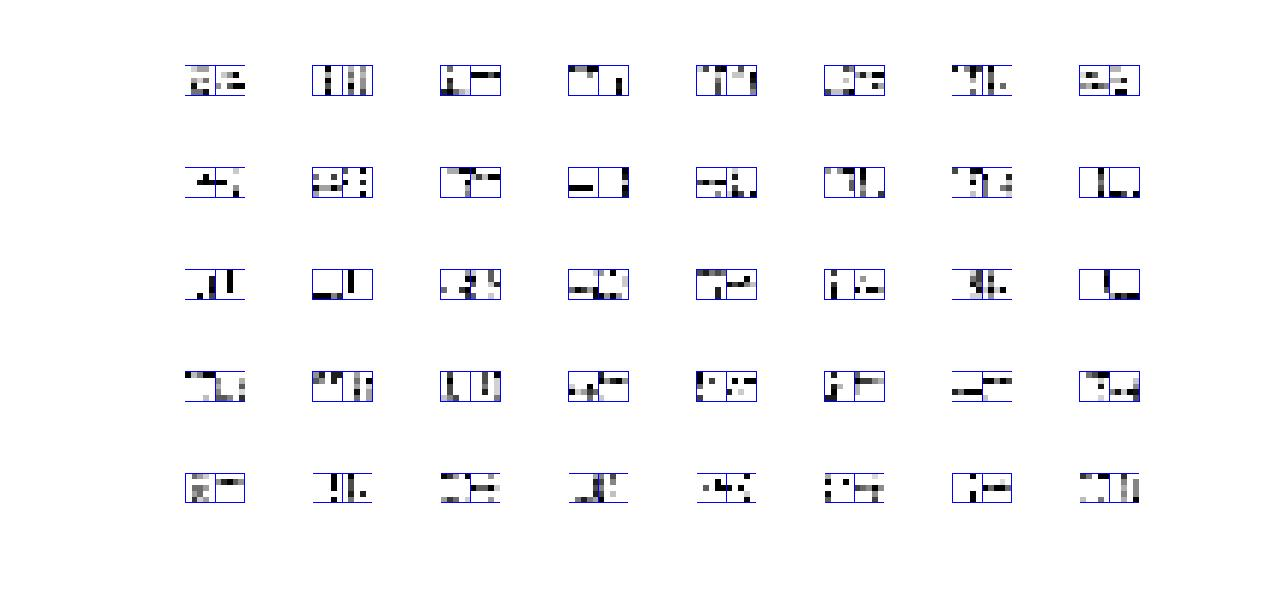
\includegraphics[width=7in,height=3in]{greedy.jpg} 
    \caption{Initialization with greedy approximation}
\end{figure}
\begin{figure}
    \centering 
    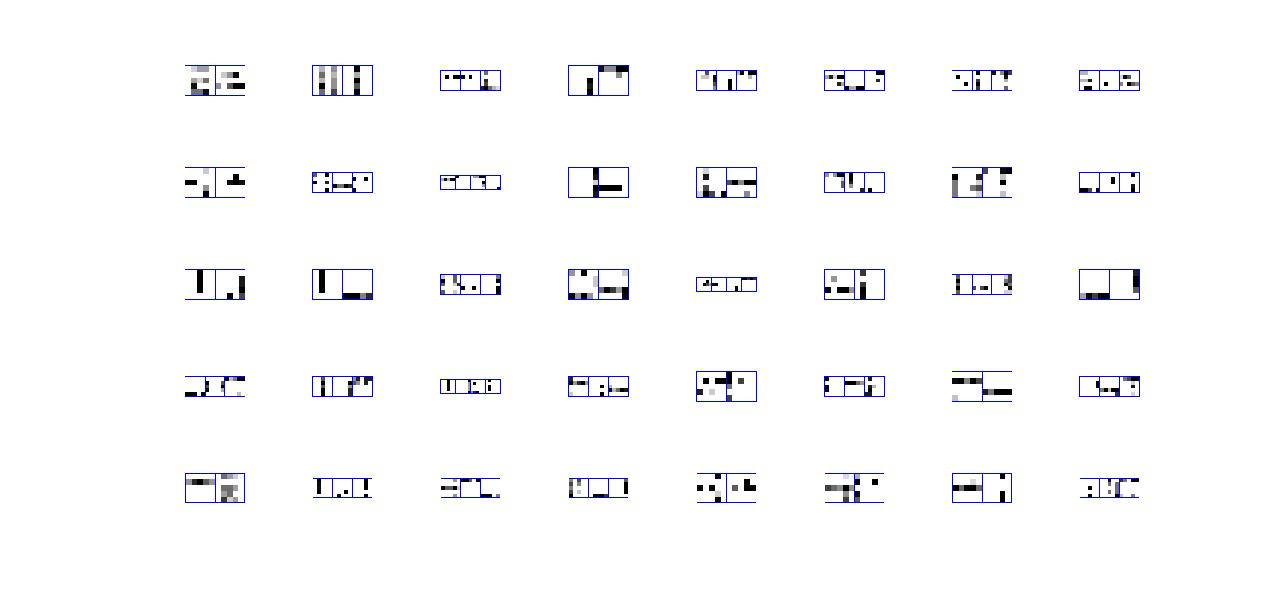
\includegraphics[width=7in,height=3in]{greedy_split.jpg} 
    \caption{Split table after Initialization}
\end{figure}



\section{3) Search}
\subsection{3.0) Statistics}
In general, we are starting from initial guess of the statistics and want it move to the ground truth.\\ \\
Sufficient Statistics: $\{t_{ji}\},\{k_{jt}\}\Longrightarrow$Local Search table/dish\\ \\
Statistics: $\{m_{j.}\},K\Longrightarrow$Split/Merge table/dish\\ \\
\subsection{3.1) Bigger Moves}
Imitate the Initialization that:\\
1) Do the move statically instead of sequentially\\
2) 
\begin{enumerate}
\item New config for tables in Restaurant j:Split all the tables in Restaurant j+local search t,k+merge t
\item New config for tables in Dish k: Split all the tables in Dish k+local search t,k
\item New config for dishes: Split all the dishes
\end{enumerate}
\subsection{3.2) Stochastic Search}
Some split-table moves are bad simply because other similar tables in the same dish do not let it go.\\
Instead of creating chaos by Bigger moves, simply we can give split move some probability to "tunnel" through the well.\\
\end{spacing}
\end{document}

%%%%%%%%%%%%%%%%%%%%%%%%%%%%%%%%%%%%%%%%%%%%%%%%%%%%%%%%%%%%%
